\section{Objectives}
Complete Lab 23 from PDF pages 91--93, including the 2-to-4 load comparison, 3-to-8 design and both 8-to-256 architectures, with every output checked.

\section{Specification Mapping}
S denotes simulated checks; D denotes analytical discussion.

\small\begin{longtable}{p{.46\linewidth}p{.30\linewidth}p{.15\linewidth}}\toprule
Requirement and PDF pages & Deck / check & Status \\ \midrule\endhead
NAND/NOR 2-to-4, 10fF (91--93) & D01/C0 & S \\
Increasing load and stage-count question (93) & D01/C1--3 & S+D \\
Design 3-to-8 (93) & D02; 8 codes & S \\
Two/three-stage 8-to-256 (93) & D03; 256 codes each & S \\
Hierarchical delay/power comparison (93) & D04; 10/100fF & S+D \\
\bottomrule\end{longtable}\normalsize


\section{Circuit and Design Derivation}
The NAND 2-to-4 uses four NAND2 gates and four output inverters; the NOR version uses four NOR2 gates. Each has two input inverters, giving 28/20 MOS devices. The primary load is 10 fF per output. The 3-to-8 uses eight NAND3/inverter pairs and three input inverters, totaling 70 MOS devices.

The two-stage 8-to-256 separately decodes low/high 4-bit groups into 16 lines each, then combines them with 256 AND2 outputs. The three-stage design starts with four 2-to-4 groups, combines them into two 4-to-16 groups, then uses final AND2 gates. Stage count refers to logical decomposition; each positive AND uses NAND+inverter, giving four/six electrical gate levels excluding input inversion. Complemented-input paths add one inverter, giving five/seven levels. Counts including input inversions are 1872/1840 MOS. Intermediate four-bit combination gates are twice unit size to drive 16 final loads. Other unit $W_p/W_n/L=3.6/1.8/0.25\,\mu$m; series NMOS/PMOS widths scale with stack length.

\section{Simulation Setup}
The model is supplied separately on the user's computer. These are 1 V, 27 $^\circ$C teaching conditions; the handout's old-process 2.5 V numbers are not pass thresholds. Actual PrimeSim HSPICE S-2021.09 runs use \texttt{accurate}, \texttt{runlvl=5} and \texttt{.print/.measure} data. Every \texttt{.alter} resets baseline parameters and temperature. All cases completed without errors or failed measurements; model and convergence notices may remain. Public netlists retain only \texttt{* MODEL\_SETUP\_REQUIRED}, with no model path. Full data are under the lab's \texttt{results/}; large files are split by deck and indexed by \texttt{simulation\_data.json}.

Four decks contain eight cases. The 2-to-4 repeats codes 0/1/2/3, 2 ns per code with 20 ps edges, at 10/50/100/500 fF and at most 1 ps steps. One-hot outputs are checked at 80\% of each slot against 0.1/0.9 V rails. DATA DC sweeps print every input code and every output for the 3-to-8 and both 8-to-256 circuits. The hierarchical transient uses codes 0,1,0,15,255,0,16,0 at 5 ns/code with at most 2 ps steps; delay explicitly measures output1 for 0-to-1 and 1-to-0.

\section{Results and Specification Checks}
\begin{center}\small\begin{tabular}{lrrrr}\toprule
Load (fF) & NAND rise/fall (ps) & NOR rise/fall (ps) & NAND/NOR P ($\mu$W) & Fails \\ \midrule
10 & 112.4/156.1 & 155.0/62.6 & 54.8/55.6 & 0 \\
50 & 213.9/201.9 & 254.0/107.6 & 76.2/77.8 & 0 \\
100 & 331.7/248.1 & 371.4/156.7 & 101.9/103.6 & 0 \\
500 & 1259.8/396.7 & 1289.6/236.6 & 237.5/233.7 & 16 \\
\bottomrule\end{tabular}\end{center}

\begin{figure}[htbp]\centering
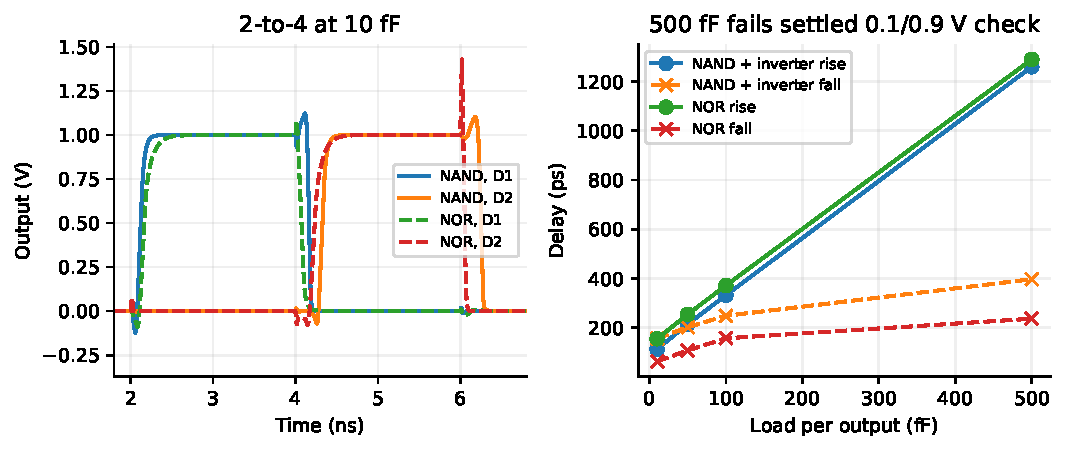
\includegraphics[width=\linewidth]{figures/decoder_load.pdf}
\caption{2-to-4 waveforms and loading; 500 fF misses settled rail criteria at the specified 2 ns code width.}
\end{figure}
\begin{center}\small\begin{tabular}{lrrrr}\toprule
Load (fF) & Stages & $t_{rise}$ (ps) & $t_{fall}$ (ps) & $P$ ($\mu$W) \\ \midrule
10 & 2 & 744.7 & 590.3 & 522.7 \\
10 & 3 & 1360.2 & 924.9 & 238.8 \\
100 & 2 & 964.9 & 693.7 & 552.7 \\
100 & 3 & 1579.8 & 1028.3 & 257.1 \\
\bottomrule\end{tabular}\end{center}

\begin{figure}[htbp]\centering
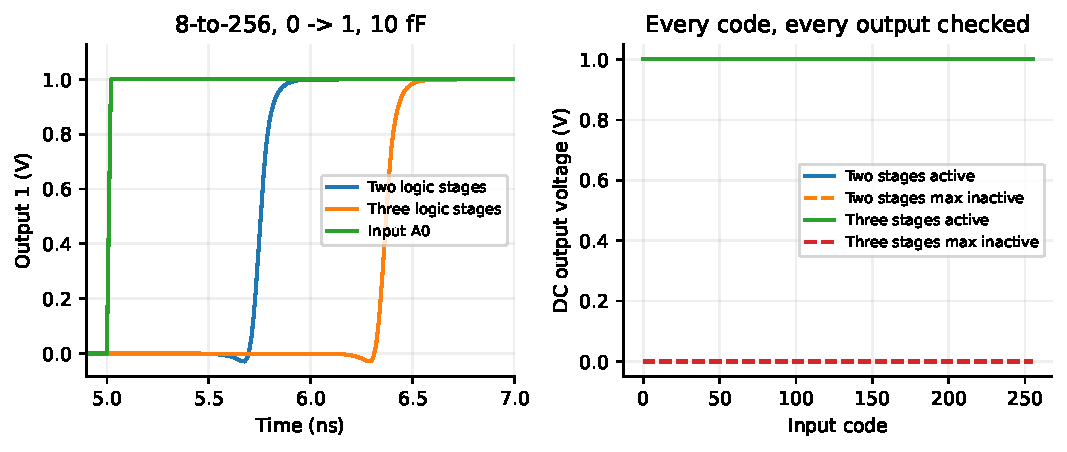
\includegraphics[width=\linewidth]{figures/hierarchical_decoder.pdf}
\caption{Representative 8-to-256 transition and exhaustive DC checks of every code and output.}
\end{figure}
All eight 3-to-8 codes pass. Each hierarchical design passes all 256 codes and every output, totaling 512 architecture/code checks. The large DC network prints convergence retries but ultimately completes and passes every truth check; no failed codes were removed.

The 2-to-4 passes all settled checks at 10/50/100 fF. At 500 fF, 16 of 18 architecture/slot checks miss the 0.1/0.9 V rails, so valid output at this code rate is not claimed. A measurable 50\% propagation delay is different from reaching full logic rails.

\section{Discussion}
More stages do not invariably mean more delay at fixed load: added buffers can distribute fanout and improve transitions, but add intrinsic delay and capacitance. Here the 10 fF two-stage rise delay is about 744.7 ps versus 1360.2 ps for three stages. Three stages use less supply power for this stimulus, 238.8 versus 522.7 $\mu$W. These are not universal speed/power rules; sizing, stack resistance, capacitance, fanout and activity change the ordering.

Despite its extra level, the NAND 2-to-4 rises faster here, while NOR falls faster; one edge cannot summarize all timing. Simultaneous input-bit changes produce hazards; truth checks apply after settling, and timing plots retain spikes. No interconnect, extracted parasitics or layout is included, so device counts only describe topology cost.

\section{Conclusion}
All three decoder scales in the handout are complete, including exhaustive 256-code checks. Heavy-load failures and dynamic hazards remain explicit. Two/three-stage comparisons apply to the stated decomposition, sizes, loads and activity.
